\documentclass{article}
\usepackage[spanish]{babel}
\usepackage[utf8]{inputenc}
\usepackage[T1]{fontenc}
\usepackage{graphicx}
\usepackage{listings}
\lstset{language=R, breaklines=true}
\usepackage{amsmath}
\usepackage{subcaption}
\usepackage[left=4cm,right=4cm]{geometry}
\usepackage[numbers,sort&compress]{natbib}


\title{\bf Práctica 9: interacciones entre partículas}
\date{\today}
\author{C. A. Estrada}

\begin{document}

\maketitle

\section{Objetivo}
Agregar a cada partícula una masa que cause fuerzas gravitacionales \cite{dra}, además de las fuerzas causadas por las cargas, y estudiar la distribución de las velocidades de las partículas verificando la relación entre la velocidad, la magnitud de la carga, la masa y las posiciones.

\section{Metodología}
Se emplea el paquete estadístico R versión 4.0.2 \cite{R} para la generación del código, utilizando el código previamente reportado para las interacciones entre partículas \cite{dra, ang}. Se utilizan 50 partículas para la simulación, donde la masa se añade al marco de datos con una distribución normal, y posteriormente se normaliza para que se obtengan partículas de masa entre 0.1 y 1, evitando masas de valor cero.
\begin{lstlisting}
p = data.frame(x = rnorm(n), y=rnorm(n), c=rnorm(n), m=rnorm(n))
mmax = max(p$m)
mmin = min(p$m)
p$m = (p$m - mmin)/(mmax - mmin)+0.1 #Masas entre 0.1 y 1
\end{lstlisting}

De manera similar, se añade la variable masa a la función de fuerza, y se toma como consideración la interacción de la masa sobre la fuerza de atracción de las partículas con base en la segunda ley de Newton, $F=ma$, por lo que se dividen las fuerzas obtenidas al final de la función fuerza entre la masa correspondiente: 
\begin{lstlisting}
return(c(fx, fy)/(mi)) 
\end{lstlisting}

Respecto a la velocidad, se considera como el cambio de posición en el tiempo (un paso), por lo que es equivalente a la distancia euclidiana entre los dos puntos en $x$ y en $y$, realizando un proceso de interacción de las partículas de cincuenta pasos en total.
\begin{lstlisting}
p$x <- foreach(i = 1:n, .combine=c) %dopar% max(min(p[i,]$x + delta * f[c(TRUE, FALSE)][i], 1), 0)
p$y <- foreach(i = 1:n, .combine=c) %dopar% max(min(p[i,]$y + delta * f[c(FALSE, TRUE)][i], 1), 0)
v = foreach(i=1:n,.combine=c)%dopar% sqrt((delta*f[c(TRUE,FALSE)][i])^2+(delta*f[c(FALSE,TRUE)][i])^2)
\end{lstlisting}

Finalmente, para observar la relación entre cada una de las variables se genera una matriz de dispersión con el paquete ``Psych'' en R \cite{psy}, que genera un diagrama de dispersión para cada par de variables, el histograma de cada una de ellas y el coeficiente de  correlación de Pearson.

\section{Resultados y discusión}
En la figura \ref{partículas} se presentan las posiciones de las partículas generadas en cuatro pasos a lo largo del proceso de interacción entre ellas, en donde comienzan estando dispersas, mientras que para el final de la simulación, la mayoría de las partículas se aglomeran por la atracción ejercida entre ellas.

\begin{figure}
\centering
\begin{subfigure}[b]{0.49\linewidth}
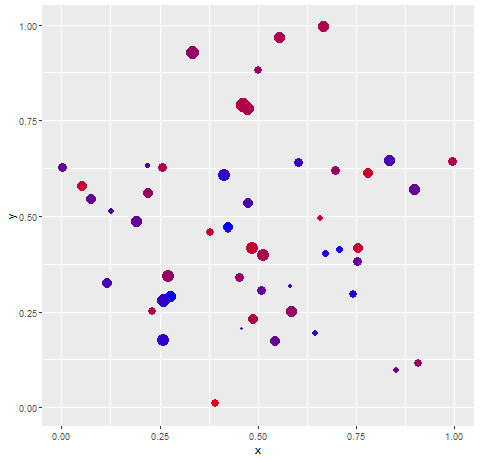
\includegraphics[width=\linewidth]{p9-t01.png}
\caption{Paso 1.}
\label{1}
\end{subfigure}
\begin{subfigure}[b]{0.49\linewidth}
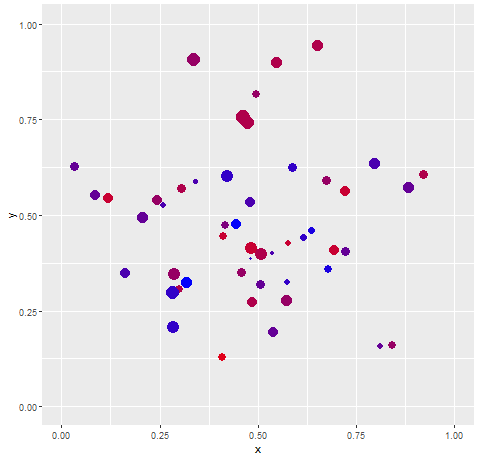
\includegraphics[width=\linewidth]{p9-t10.png}
\caption{Paso 10.}
\label{2}
\end{subfigure}
\begin{subfigure}[b]{0.49\linewidth}
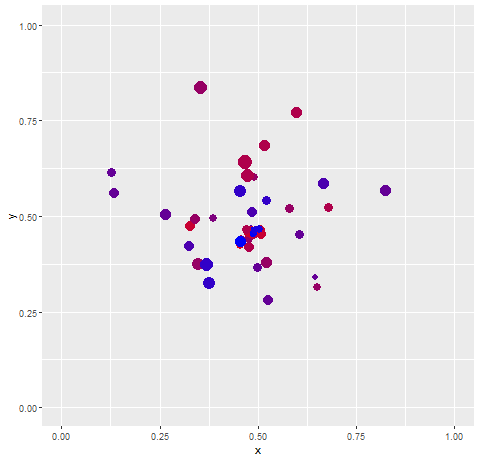
\includegraphics[width=\linewidth]{p9-t25.png}
\caption{Paso 25.}
\label{3}
\end{subfigure}
\begin{subfigure}[b]{0.49\linewidth}
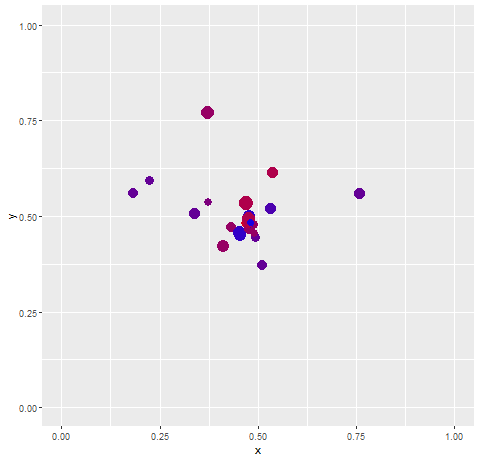
\includegraphics[width=\linewidth]{p9-t50.png}
\caption{Paso 50.}
\label{4}
\end{subfigure}
\caption{Posicionamiento de las partículas en diferentes pasos del proceso de interacción.}
\label{partículas}
\end{figure}

En las figuras \ref{matriz} y \ref{matriz2} se presentan las matrices de dispersión para las cinco variables empleadas: posición en $x$, posición en $y$, carga, masa y velocidad. En la figura \ref{matriz} se observa que para los pasos 1 y 10 del proceso de interacción se comienza con una gran dispersión de las partículas, como se muestra en los histogramas para la posición en $x$ y en $y$, en donde las únicas correlaciones significativas (valores de correlación con estrellas) son aquellas entre la masa y la velocidad, y también, aunque en menor medida, entre la masa y la posición en $y$.

\begin{figure}
\centering
\begin{subfigure}[b]{0.7\linewidth}
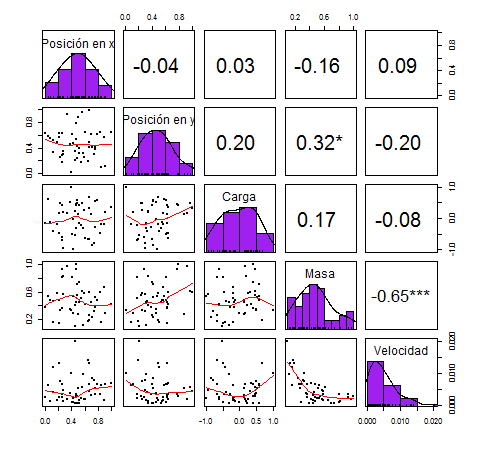
\includegraphics[width=\linewidth]{p9-mat01.png}
\caption{Paso 1.}
\label{5}
\end{subfigure}
\begin{subfigure}[b]{0.7\linewidth}
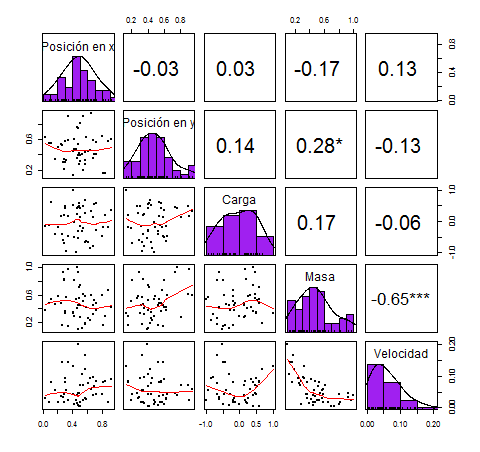
\includegraphics[width=\linewidth]{p9-mat10.png}
\caption{Paso 10.}
\label{6}
\end{subfigure}
\caption{Matrices de dispersión de las partículas en función de las diferentes variables en los pasos 1 y 10 del proceso de interacción.}
\label{matriz}
\end{figure}

En los histogramas de la figura \ref{matriz2} se observa que para los pasos 25 y 50 las posiciones en $x$ y en $y$ tienden a quedarse aproximadamente en la posición de 0.4 para ambas coordenadas, y que se presenta un aumento en la correlación entre ambas variables, aunque sin llegar a ser significativo. Además, al finalizar la simulación, la única correlación significativa se presenta entre la masa y la velocidad, siendo una correlación negativa de -0.64, mientras que hubo un decremento en la correlación aparente entre la masa y la posición en $y$ que se observa en los pasos 1, 10 y 25. Por otra parte, la influencia de la carga sobre las demás variables parece no tener ningún efecto significativo en ninguno de los pasos de la simulación. 

\begin{figure}
\centering
\begin{subfigure}[b]{0.7\linewidth}
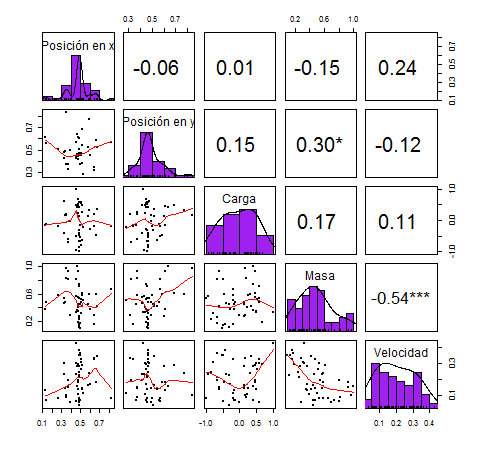
\includegraphics[width=\linewidth]{p9-mat25.png}
\caption{Paso 25.}
\label{7}
\end{subfigure}
\begin{subfigure}[b]{0.7\linewidth}
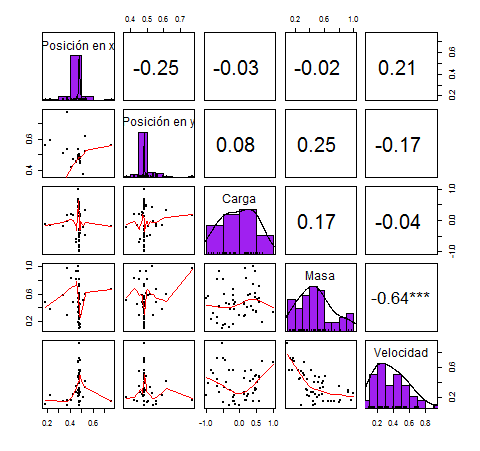
\includegraphics[width=\linewidth]{p9-mat50.png}
\caption{Paso 50.}
\label{8}
\end{subfigure}
\caption{Matrices de dispersión de las partículas en función de las diferentes variables en los pasos 25 y 50 del proceso de interacción.}
\label{matriz2}
\end{figure}

\section{Conclusión}
La influencia de la masa de las partículas sobre la velocidad es la más significativa a lo largo del proceso de interacción, estando inversamente relacionadas. 

\bibliography{P9}
\bibliographystyle{unsrtnat}

\end{document}



